% LangLLM: IEEE BigData 2026 High School Symposium submission.
% Compile with pdfLaTeX. All numbers come from numbers.tex (generated by
% `python -m langllm.paper_numbers` from results/); do not type numbers by hand.
\documentclass[conference]{IEEEtran}
\IEEEoverridecommandlockouts
\usepackage[utf8]{inputenc}
\usepackage[T1]{fontenc}
\usepackage{amsmath,amssymb}
\usepackage{graphicx}
\usepackage{booktabs}
\usepackage{multirow}
\usepackage{url}
\usepackage[hidelinks]{hyperref}
\usepackage{xcolor}
% GENERATED by python -m langllm.paper_numbers from results/. Do not edit by hand.
% Rounding: half-up. Accuracies as .xxx, percentages as xx.x\%.
\newcommand{\NResponses}{839}
\newcommand{\NCollected}{840}
\newcommand{\NTranslations}{1,440}
\newcommand{\NJudgments}{4195}
\newcommand{\NPrompts}{12}
\newcommand{\NLangs}{7}
\newcommand{\NModels}{5}
\newcommand{\NFeatures}{21}
\newcommand{\Chance}{20\%}
\newcommand{\LRen}{.717}
\newcommand{\LRloen}{.61}
\newcommand{\LRhien}{.82}
\newcommand{\Foneen}{.711}
\newcommand{\RFen}{.675}
\newcommand{\LRes}{.625}
\newcommand{\LRloes}{.53}
\newcommand{\LRhies}{.70}
\newcommand{\Fonees}{.625}
\newcommand{\RFes}{.675}
\newcommand{\LRzh}{.650}
\newcommand{\LRlozh}{.55}
\newcommand{\LRhizh}{.73}
\newcommand{\Fonezh}{.644}
\newcommand{\RFzh}{.650}
\newcommand{\LRru}{.650}
\newcommand{\LRloru}{.52}
\newcommand{\LRhiru}{.78}
\newcommand{\Foneru}{.654}
\newcommand{\RFru}{.717}
\newcommand{\LRja}{.708}
\newcommand{\LRloja}{.63}
\newcommand{\LRhija}{.78}
\newcommand{\Foneja}{.707}
\newcommand{\RFja}{.733}
\newcommand{\LRtr}{.592}
\newcommand{\LRlotr}{.50}
\newcommand{\LRhitr}{.69}
\newcommand{\Fonetr}{.596}
\newcommand{\RFtr}{.600}
\newcommand{\LRhi}{.639}
\newcommand{\LRlohi}{.56}
\newcommand{\LRhihi}{.71}
\newcommand{\Fonehi}{.634}
\newcommand{\RFhi}{.622}
\newcommand{\LRmin}{.59}
\newcommand{\LRmax}{.72}
\newcommand{\LRminPct}{59\%}
\newcommand{\LRmaxPct}{72\%}
\newcommand{\RFmin}{.60}
\newcommand{\RFmax}{.73}
\newcommand{\ClusterCIminLo}{.50}
\newcommand{\ClusterCIhalfwidth}{9}
\newcommand{\LRlenMin}{.44}
\newcommand{\LRlenMax}{.57}
\newcommand{\RFlenMin}{.66}
\newcommand{\RFlenMax}{.78}
\newcommand{\RecallgptMin}{67\%}
\newcommand{\RecallgptMax}{92\%}
\newcommand{\RecallgeminiMin}{54\%}
\newcommand{\RecallgeminiMax}{75\%}
\newcommand{\RecallclaudeMin}{63\%}
\newcommand{\RecallclaudeMax}{79\%}
\newcommand{\RecallgrokMin}{63\%}
\newcommand{\RecallgrokMax}{88\%}
\newcommand{\RecalldeepseekMin}{25\%}
\newcommand{\RecalldeepseekMax}{58\%}
\newcommand{\TopCoefFeatures}{paragraph count, comma rate, char-bigram entropy, paragraph length, Zipf slope}
\newcommand{\PooledTopFive}{paragraph count, paragraph length, sentence length, comma rate, hapax rate}
\newcommand{\Judgegpt}{20.6\%}
\newcommand{\JudgegptOwn}{82\%}
\newcommand{\JudgegptFalse}{82\%}
\newcommand{\JudgegptFisherP}{$p = 0.583$}
\newcommand{\JudgegptSelfClaim}{82\%}
\newcommand{\Judgegemini}{21.2\%}
\newcommand{\JudgegeminiOwn}{3\%}
\newcommand{\JudgegeminiFalse}{4\%}
\newcommand{\JudgegeminiFisherP}{$p = 0.844$}
\newcommand{\JudgegeminiSelfClaim}{4\%}
\newcommand{\Judgeclaude}{25.4\%}
\newcommand{\JudgeclaudeOwn}{17\%}
\newcommand{\JudgeclaudeFalse}{7\%}
\newcommand{\JudgeclaudeFisherP}{$p < 10^{-4}$}
\newcommand{\JudgeclaudeSelfClaim}{9\%}
\newcommand{\Judgegrok}{21.9\%}
\newcommand{\JudgegrokOwn}{0\%}
\newcommand{\JudgegrokFalse}{0\%}
\newcommand{\JudgegrokFisherP}{$p = 1.000$}
\newcommand{\JudgegrokSelfClaim}{0\%}
\newcommand{\Judgedeepseek}{20.3\%}
\newcommand{\JudgedeepseekOwn}{7\%}
\newcommand{\JudgedeepseekFalse}{8\%}
\newcommand{\JudgedeepseekFisherP}{$p = 0.806$}
\newcommand{\JudgedeepseekSelfClaim}{8\%}
\newcommand{\JudgeMin}{20.3\%}
\newcommand{\JudgeMax}{25.4\%}
\newcommand{\JudgeMeanen}{.230}
\newcommand{\JudgeBesten}{.267}
\newcommand{\JudgeBestNameen}{Claude Opus 4.7}
\newcommand{\JudgeMeanes}{.207}
\newcommand{\JudgeBestes}{.217}
\newcommand{\JudgeBestNamees}{Grok 4.3}
\newcommand{\JudgeMeanzh}{.208}
\newcommand{\JudgeBestzh}{.233}
\newcommand{\JudgeBestNamezh}{Claude Opus 4.7}
\newcommand{\JudgeMeanru}{.237}
\newcommand{\JudgeBestru}{.258}
\newcommand{\JudgeBestNameru}{Gemini 3.5 Flash}
\newcommand{\JudgeMeanja}{.198}
\newcommand{\JudgeBestja}{.225}
\newcommand{\JudgeBestNameja}{Claude Opus 4.7}
\newcommand{\JudgeMeantr}{.205}
\newcommand{\JudgeBesttr}{.258}
\newcommand{\JudgeBestNametr}{Claude Opus 4.7}
\newcommand{\JudgeMeanhi}{.247}
\newcommand{\JudgeBesthi}{.361}
\newcommand{\JudgeBestNamehi}{Claude Opus 4.7}
\newcommand{\GapJudgeMin}{28}
\newcommand{\GapJudgeMax}{48}
\newcommand{\GapJudgeMeanMin}{39}
\newcommand{\GapJudgeMeanMax}{51}
\newcommand{\ClaudeOwnen}{25\%}
\newcommand{\ClaudeOwnCIen}{[10\%, 47\%]}
\newcommand{\ClaudeOwnes}{0\%}
\newcommand{\ClaudeOwnCIes}{[0\%, 14\%]}
\newcommand{\ClaudeOwnzh}{8\%}
\newcommand{\ClaudeOwnCIzh}{[1\%, 27\%]}
\newcommand{\ClaudeOwnru}{0\%}
\newcommand{\ClaudeOwnCIru}{[0\%, 14\%]}
\newcommand{\ClaudeOwnja}{38\%}
\newcommand{\ClaudeOwnCIja}{[19\%, 59\%]}
\newcommand{\ClaudeOwntr}{8\%}
\newcommand{\ClaudeOwnCItr}{[1\%, 27\%]}
\newcommand{\ClaudeOwnhi}{42\%}
\newcommand{\ClaudeOwnCIhi}{[22\%, 63\%]}
\newcommand{\ClaudeHindiAcc}{36.1\%}
\newcommand{\ClaudeEnglishAcc}{26.7\%}
\newcommand{\NGen}{.750}
\newcommand{\NGloen}{.71}
\newcommand{\NGhien}{.79}
\newcommand{\WGen}{.783}
\newcommand{\NGes}{.733}
\newcommand{\NGloes}{.65}
\newcommand{\NGhies}{.80}
\newcommand{\WGes}{.783}
\newcommand{\NGzh}{.867}
\newcommand{\NGlozh}{.81}
\newcommand{\NGhizh}{.93}
\newcommand{\WGzh}{.558}
\newcommand{\NGru}{.783}
\newcommand{\NGloru}{.66}
\newcommand{\NGhiru}{.88}
\newcommand{\WGru}{.825}
\newcommand{\NGja}{.792}
\newcommand{\NGloja}{.71}
\newcommand{\NGhija}{.87}
\newcommand{\WGja}{.683}
\newcommand{\NGtr}{.783}
\newcommand{\NGlotr}{.73}
\newcommand{\NGhitr}{.84}
\newcommand{\WGtr}{.833}
\newcommand{\NGhi}{.782}
\newcommand{\NGlohi}{.73}
\newcommand{\NGhihi}{.83}
\newcommand{\WGhi}{.731}
\newcommand{\NGmin}{.73}
\newcommand{\NGmax}{.87}
\newcommand{\NGmean}{.78}
\newcommand{\WGmean}{.74}
\newcommand{\GapNGmin}{3}
\newcommand{\GapNGmax}{22}
\newcommand{\NGsigLangs}{Chinese, Turkish}
\newcommand{\NGsigN}{2}
\newcommand{\HolmN}{28}
\newcommand{\FeatVsChanceAllSig}{all seven}
\newcommand{\FeatVsJudgeAllSig}{all seven}
\newcommand{\NGrho}{0.32}
\newcommand{\NGrhoP}{$p = 0.478$}
\newcommand{\NGglmBeta}{+0.025}
\newcommand{\NGglmP}{$p = 0.380$}
\newcommand{\Beta}{-0.038}
\newcommand{\BetaSE}{0.042}
\newcommand{\BetaLo}{-0.12}
\newcommand{\BetaHi}{+0.04}
\newcommand{\BetaP}{$p = 0.361$}
\newcommand{\SteepestDeclinePts}{17}
\newcommand{\SteepestDeclineAcc}{.55}
\newcommand{\BetaLen}{-0.053}
\newcommand{\BetaLenP}{$p = 0.164$}
\newcommand{\RhoRQtwo}{-0.45}
\newcommand{\RhoRQtwoP}{$p = 0.310$}
\newcommand{\BetaLangSE}{0.032}
\newcommand{\BetaLangP}{$p = 0.226$}
\newcommand{\BetaLangPromptSE}{0.040}
\newcommand{\BetaLangPromptP}{$p = 0.343$}
\newcommand{\EtaModel}{.145}
\newcommand{\EtaLang}{.54}
\newcommand{\EtaInter}{.13}
\newcommand{\EtaPrompt}{.16}
\newcommand{\EtaModelmeantokenlen}{.11}
\newcommand{\EtaLangmeantokenlen}{.99}
\newcommand{\EtaModelfuncwordratio}{.11}
\newcommand{\EtaLangfuncwordratio}{.94}
\newcommand{\EtaModelhapaxrate}{.38}
\newcommand{\EtaLanghapaxrate}{.93}
\newcommand{\EtaModelzipfslope}{.37}
\newcommand{\EtaLangzipfslope}{.93}
\newcommand{\EtaModelmattr}{.10}
\newcommand{\EtaLangmattr}{.88}
\newcommand{\EtaModelcommaper1k}{.32}
\newcommand{\EtaLangcommaper1k}{.62}
\newcommand{\EtaModelbigramentropy}{.31}
\newcommand{\EtaLangbigramentropy}{.97}
\newcommand{\EtaModelparacount}{.29}
\newcommand{\EtaLangparacount}{.12}
\newcommand{\EtaModelsubordrate}{.01}
\newcommand{\EtaLangsubordrate}{.77}
\newcommand{\EtaModelquestionrate}{.01}
\newcommand{\EtaLangquestionrate}{.07}
\newcommand{\EtaModeldepdepth}{.03}
\newcommand{\EtaLangdepdepth}{.41}
\newcommand{\EtaModelSmallMax}{.03}
\newcommand{\TransferOff}{.49}
\newcommand{\TransferDiag}{.65}
\newcommand{\TransferMin}{.37}
\newcommand{\TransferMax}{.59}
\newcommand{\TransferSig}{42}
\newcommand{\TransferRatio}{74\%}
\newcommand{\NGTransferOff}{.28}
\newcommand{\NGTransferSig}{14}
\newcommand{\NGTransferConst}{14}
\newcommand{\NGTransferMax}{.50}
\newcommand{\NGFairOff}{.41}
\newcommand{\NGFairAbove}{41}
\newcommand{\PunctDiag}{.62}
\newcommand{\PunctOff}{.38}
\newcommand{\CentEn}{3.59}
\newcommand{\CentHi}{2.69}
\newcommand{\CentRho}{-0.96}
\newcommand{\CentP}{$p = 4.5e-04$}
\newcommand{\BWen}{.41}
\newcommand{\BWhi}{.18}
\newcommand{\BWrho}{-1.00}
\newcommand{\SilEn}{0.04}
\newcommand{\SilHi}{-0.02}
\newcommand{\SilRho}{-0.93}
\newcommand{\SilP}{$p = 0.003$}
\newcommand{\CentCIsep}{yes}
\newcommand{\CentHiCIhi}{2.81}
\newcommand{\CentEnCIlo}{3.12}
\newcommand{\BWCIsep}{yes}
\newcommand{\BWHiCIhi}{0.19}
\newcommand{\BWEnCIlo}{0.26}
\newcommand{\SilCIsep}{no}
\newcommand{\SilHiCIhi}{-0.02}
\newcommand{\SilEnCIlo}{-0.02}
\newcommand{\PairclaudegrokEn}{5.42}
\newcommand{\PairclaudegrokHi}{3.46}
\newcommand{\PairdeepseekgrokEn}{4.86}
\newcommand{\PairdeepseekgrokHi}{2.02}
\newcommand{\PairgptgrokEn}{5.69}
\newcommand{\PairgptgrokHi}{2.69}
\newcommand{\PairgeminigrokEn}{3.55}
\newcommand{\PairgeminigrokHi}{2.96}
\newcommand{\PairLargestEn}{gpt--grok (5.69), claude--grok (5.42), deepseek--grok (4.86)}
\newcommand{\TrGoogleMin}{.57}
\newcommand{\TrGoogleMax}{.66}
\newcommand{\TrGoogleMean}{.625}
\newcommand{\TrGoogleTrainEn}{.664}
\newcommand{\TrGoogleTrainNative}{.521}
\newcommand{\TrGoogleEtaBefore}{.40}
\newcommand{\TrGoogleEtaAfter}{.32}
\newcommand{\TrGoogleRhoAbove}{16}
\newcommand{\TrLLMMin}{.59}
\newcommand{\TrLLMMax}{.70}
\newcommand{\TrLLMMean}{.629}
\newcommand{\TrLLMTrainEn}{.660}
\newcommand{\TrLLMTrainNative}{.531}
\newcommand{\TrLLMEtaBefore}{.40}
\newcommand{\TrLLMEtaAfter}{.30}
\newcommand{\TrLLMRhoAbove}{16}
\newcommand{\TrAllMin}{.57}
\newcommand{\TrAllMax}{.70}
\newcommand{\TrNativeMean}{.644}
\newcommand{\TrLLMHiTrainEn}{.77}
\newcommand{\Survparacount}{1.00}
\newcommand{\Survparalenmean}{.98}
\newcommand{\Survsentlenmean}{.89}
\newcommand{\Survburstiness}{.87}
\newcommand{\Survmattr}{.32}
\newcommand{\Survfuncwordratio}{.46}
\newcommand{\Survbigramentropy}{.49}
\newcommand{\NGTrLopoMean}{.72}
\newcommand{\NGTrLopoMin}{.63}
\newcommand{\NGTrLopoMax}{.78}
\newcommand{\NGTrTrainEnNonLatinMin}{.21}
\newcommand{\NGTrTrainEnNonLatinMax}{.24}
\newcommand{\NGTrTrainEnEs}{.57}
\newcommand{\NGTrTrainEnMean}{.29}
\newcommand{\TrTrainEnMin}{.58}
\newcommand{\TrTrainEnMax}{.72}
\newcommand{\CurveKfiveMin}{.50}
\newcommand{\CurveKfiveMax}{.75}
\newcommand{\CurveKtenWithin}{9}
\newcommand{\CurveJaPeakK}{7}
\newcommand{\CurveJaPeakF1}{.79}
\newcommand{\AblMaxDrop}{.11}
\newcommand{\AblStructMin}{.31}
\newcommand{\AblStructMax}{.61}
\newcommand{\AblPunctMin}{.26}
\newcommand{\AblPunctMax}{.53}
\newcommand{\AblLexMin}{.33}
\newcommand{\AblLexMax}{.55}

\graphicspath{{figures/}}

\begin{document}

\title{Do LLM Fingerprints Survive Outside English?\\
\large Interpretable Attribution of Five Frontier Models Across Seven Languages}

\author{
\IEEEauthorblockN{Adrian Erlikhman}
\IEEEauthorblockA{\textit{High School Student}\\
\textit{Los Angeles Center for Enriched Studies}\\
Los Angeles, CA, USA\\
erlikhman.adrian@gmail.com}
\and
\IEEEauthorblockN{Michael Tarekegn}
\IEEEauthorblockA{\textit{High School Student}\\
\textit{Los Angeles Center for Enriched Studies}\\
Los Angeles, CA, USA}
\and
\IEEEauthorblockN{Philo Juang}
\IEEEauthorblockA{\textit{University of California, Los Angeles}\\
Los Angeles, CA, USA}
}

\maketitle

\begin{abstract}
Tools that attribute AI-generated text to the model that wrote it are built and evaluated mostly in English, while the settings where attribution matters, such as disinformation tracing and content moderation, are multilingual. We ask whether the stylistic fingerprint of a specific large language model (LLM) survives outside English, and whether an interpretable representation can carry it. We collected \NCollected{} persuasive essays from five frontier models (GPT-5.5, Gemini 3.5 Flash, Claude Opus 4.7, Grok 4.3, DeepSeek V4 Pro) in seven languages ordered by training-data resource level, holding content fixed with natively authored prompts, and described each text by \NFeatures{} features defined on Universal Dependencies so that every feature has the same meaning in every language. A logistic-regression classifier attributes texts five ways at \LRmin{}--\LRmax{} accuracy in every language (chance \Chance{}, leave-one-prompt-out), and accuracy does not decline with resource level: the fitted gradient is \Beta{} log-odds per rank step (95\% CI \BetaLo{} to \BetaHi{}). A character $n$-gram classifier is \GapNGmin{}--\GapNGmax{} points more accurate within a language, but the two representations part ways at language boundaries: after within-language standardization the interpretable features transfer between languages at mean accuracy \TransferOff{} against \NGFairOff{} for $n$-grams, and a classifier trained on English reads machine translations of English text at \TrGoogleTrainEn{} against \NGTrTrainEnMean{}, because paragraphing, sentence rhythm and punctuation survive translation while vocabulary does not. Models converge stylistically as resources fall (centroid separation vs.\ rank, $\rho = \CentRho{}$) without becoming indistinguishable, and the five models themselves, asked which model wrote each text, score \JudgeMin{}--\JudgeMax{}. Code, prompts, all texts and translations are released.
\end{abstract}

\begin{IEEEkeywords}
authorship attribution, AI-generated text, multilingual text mining, stylometry, large language models
\end{IEEEkeywords}

\section{Introduction}
Most work on machine-generated text asks whether a text was written by a person or by a model. A second question matters for provenance: \emph{which} model wrote it. Answering it lets an analyst link an influence campaign to a toolchain, check a vendor's claim about where its content came from, or apply platform rules that differ by provider. The attribution literature is mostly English~\cite{uchendu2020authorship,uchendu2021turingbench,sun2025idiosyncrasies}, and the two multilingual studies we know of use fine-tuned or probability-based classifiers whose decisions cannot be inspected~\cite{lacava2026multilingual}.

There are two reasons to doubt that English results carry over. First, models see far less training text in lower-resource languages~\cite{joshi2020state}, so their writing there may be less distinctive or less stable. Second, languages differ in script and morphology, so many classic stylometric measures (readability formulas, contractions, hedge lists) are undefined outside English, and the measures that are defined may track the language more than the author. Character $n$-grams, the standard strong baseline in authorship attribution~\cite{stamatatos2009survey,sapkota2015ngrams}, have the opposite problem: they are accurate but tied to the script and vocabulary of the language they were fit on.

We address both problems with a design that holds content fixed across languages and describes every text with features defined on Universal Dependencies (UD)~\cite{nivre2020ud}, and we measure what that choice costs and buys against an $n$-gram baseline. We ask six pre-registered questions. \textbf{RQ1}: Can five frontier models be told apart within each of seven languages? \textbf{RQ2}: Does attribution weaken as a language's resource level falls? \textbf{RQ3}: Is a model's fingerprint shared across languages or specific to each? \textbf{RQ4}: Do models converge on one style in lower-resource languages? \textbf{RQ5}: Does machine translation erase the fingerprint? \textbf{RQ6}: As a baseline, can the models themselves identify the author? A seventh analysis, added in response to review, asks what the interpretable representation gives up relative to $n$-grams and where it wins.

Our contributions are: (i) a content-controlled multilingual corpus of \NCollected{} essays (5 models $\times$ 7 languages $\times$ 12 prompts $\times$ 2 generations) and \NTranslations{} machine translations, released with code; (ii) a \NFeatures{}-feature representation with one definition in every language, with which five-way attribution reaches \LRmin{}--\LRmax{} in all seven languages, with no detectable resource gradient and with five features carrying most of the signal; (iii) a direct comparison with character $n$-grams showing that the opaque baseline is more accurate within a language but that only the interpretable features carry a classifier across a language or translation boundary without retraining; (iv) evidence that models converge stylistically in lower-resource languages while remaining attributable, and that LLM judges attribute at or near chance. All decision rules were written down before data collection; deviations and additions are labelled.

\section{Related Work}
\textbf{Detection.} Zero-shot detectors~\cite{mitchell2023detectgpt,hans2024binoculars} and multilingual benchmarks~\cite{macko2023multitude,wang2024m4} separate human from machine text; detectors fine-tuned on English lose about a quarter of their F1 on other languages~\cite{wang2025genaidetect}. These works ask human versus machine, not which machine, and the generator-identification subtask of SemEval-2024 Task 8 was English-only.

\textbf{Model attribution.} Uchendu et al.\ framed attribution among neural generators and built TuringBench~\cite{uchendu2020authorship,uchendu2021turingbench}; Kumarage and Liu applied stylometric features to LLM attribution~\cite{kumarage2023neural}; Sun et al.\ showed that embedding classifiers separate current model families and that the signal survives LLM translation into Chinese~\cite{sun2025idiosyncrasies}, all in English or English-centred. La Cava et al.\ attribute among seven LLMs across 18 languages with fine-tuned and probability-based detectors and report cross-lingual transfer~\cite{lacava2026multilingual}. Stylometric detection has been applied language by language with language-specific feature sets, for Japanese~\cite{zaitsu2025stylometry} and Polish~\cite{przystalski2025stylometry} among others. UD-based features have been used for cross-language attribution of human authors~\cite{murauer2021dtgrams}. To our knowledge, no prior study attributes text to its source model with features that have the same definition in every language, holds content fixed across languages, tests attribution against a resource gradient, or measures what interpretability costs against an $n$-gram baseline; see~\cite{huang2024attribution} for a survey.

\textbf{Homogenization and LLM judges.} Writing with LLMs reduces the diversity of human text~\cite{padmakumar2024diversity,sourati2026shrinking}, and a two-language benchmark compares model registers with human ones~\cite{milicka2025benchmark}; whether models converge on \emph{each other} where training data is thin has not been tested. LLM evaluators recognize and favour their own outputs~\cite{panickssery2024self}. We use LLM judges only as a baseline; a companion study examines self-recognition in English under two elicitation formats~\cite{erlikhman2026compllm}.

\section{Data and Method}
\subsection{Models, languages and prompts}
The five subject models, queried through OpenRouter with the served model string logged for every response, are GPT-5.5, Gemini 3.5 Flash, Claude Opus 4.7, Grok 4.3 and DeepSeek V4 Pro. The seven languages are English, Spanish, Chinese, Russian, Japanese, Turkish and Hindi, assigned ordinal resource ranks 1--7 in that order to reflect their approximate share of web training data~\cite{joshi2020state}; we use a rank because numeric estimates disagree by source.

Twelve English prompts each fix a topic, a stance (six for, six against), three supporting claims, a prose-only instruction and a reading-level tier. For each language a model that is not a subject (Llama 4 Maverick) wrote a native version of each prompt from those elements rather than translating the English, so the wording is idiomatic while the content is fixed. A model from a third family (Qwen 3.7 Plus) then read each of the 84 prompts blind, extracted the topic, stance and claims, and compared them with the original; prompts that failed were regenerated with the reviewer's note until all 84 passed.

\subsection{Generation, validation and features}
Each prompt was sent as a single user turn with no system prompt at temperature 0.7, twice per cell with fixed seeds and reasoning traces excluded, giving $5 \times 12 \times 7 \times 2 = \NCollected{}$ responses. Each passed language identification (confidence $\geq 0.6$), a 150--900 word-equivalent window and a per-language refusal check. One Grok response to a Hindi prompt was written in English and excluded, leaving \NResponses{} texts; ten DeepSeek responses that spent a 4,000-token budget on hidden reasoning were re-collected at 16,000.

Every text was parsed with Stanza~\cite{qi2020stanza} in all seven languages, with Chinese and Japanese pre-split on sentence-final punctuation. We compute \NFeatures{} features in five groups. \emph{Lexical}: moving-average type--token ratio (MATTR, window 50)~\cite{covington2010mattr}, hapax rate, mean token length, Zipf slope. \emph{Syntactic}: mean and SD of sentence length, burstiness~\cite{goh2008burstiness}, mean maximum dependency depth, subordinate-clause rate (\texttt{acl}, \texttt{advcl}, \texttt{ccomp}, \texttt{xcomp}, \texttt{csubj} per sentence), function-word ratio, first-person rate. \emph{Structure}: paragraph count and length, question rate, connective rate. \emph{Punctuation}: commas, colons, dashes and semicolons per 1,000 tokens, with full-width and script variants mapped to the same feature. \emph{Character}: character-bigram entropy and digit rate. English-only measures such as readability formulas, contractions and hedges are excluded.

\subsection{Analysis}
The unit of analysis is one response. The two generations of a prompt are not independent, so every cross-validation split is leave-one-prompt-out (LOPO, 12 folds) and every confidence interval and clustered standard error groups by prompt. Tests against chance are one-sided exact binomials; comparisons between classifiers on the same texts are exact McNemar tests; the 28 headline comparisons (features vs.\ chance, $n$-grams vs.\ chance, features vs.\ $n$-grams, features vs.\ the best LLM judge, in seven languages) are Holm-corrected as one family.

\textbf{RQ1.} Within each language, multinomial logistic regression on standardized features (primary, interpretable) and a random forest (ceiling), with prompt-clustered bootstrap intervals. \textbf{Baseline.} TF-IDF over character 1--4-grams fit inside each training fold, then logistic regression; word 1--2-grams likewise. \textbf{RQ2.} A binomial GLM of cell-level correctness on resource rank with clustered standard errors (by prompt, by language, and by both), plus Spearman's $\rho$ over the seven per-language accuracies; as a robustness check, features residualized on log length within each language. \textbf{RQ3.} For each feature, a two-way ANOVA (model $\times$ language, prompt as a blocking factor) with partial $\eta^2$; and a transfer matrix in which features are z-scored within each language, a classifier is trained on language $A$ and tested on $B$. For $n$-grams the fair counterpart fits the vocabulary on the union of $A$ and $B$ (no labels) and z-scores TF-IDF columns within each language, so both representations receive the same unlabelled adaptation to the target language. \textbf{RQ4.} After z-scoring within each language, the mean pairwise distance between the five model centroids, the silhouette of model labels and the between/within scatter ratio, with stratified bootstrap intervals and Spearman's $\rho$ against rank. \textbf{RQ5.} All 120 English responses were translated into the six other languages by Google Translate and by a free open model that is not a subject (MiniMax M3). We measure attribution on the translations alone, transfer from classifiers trained on the English originals or on native responses in the target language, and per-feature Spearman correlation between each original and its translation, for both representations. \textbf{RQ6.} Each subject model was shown every text without metadata and asked which of the five models wrote it, one text at a time with a candidate list, in the single-text protocol of~\cite{bai2025selfrecognition}: option order shuffled, temperature 0, hidden reasoning disabled where the API allows it. \textbf{Feature economy.} A nested feature-selection curve: within each LOPO fold, features are ranked by mean absolute standardized coefficient on the training fold only, the top $k$ are refit, and the held-out prompt is scored, for $k = 1, \dots, \NFeatures{}$; and a per-language ablation of each feature group.

\begin{table}[t]
\caption{Per-language results. LR: logistic regression on the \NFeatures{} UD features, accuracy [prompt-clustered 95\% CI]; F1: macro-F1; $n$-gram: character 1--4-gram TF-IDF [CI]; Judges: mean of the five LLM judges (best); Sep.: mean distance between model centroids ($z$-units). Chance accuracy is 0.20.}
\label{tab:main}
\centering
\small
\setlength{\tabcolsep}{3.2pt}
\begin{tabular}{l c l c l l c}
\toprule
Language & Rank & LR [95\% CI] & F1 & $n$-gram [CI] & Judges & Sep. \\
\midrule
English  & 1 & \LRen{} [\LRloen{}--\LRhien{}] & \Foneen{} & \NGen{} [\NGloen{}--\NGhien{}] & \JudgeMeanen{} (\JudgeBesten{}) & \CentEn{} \\
Spanish  & 2 & \LRes{} [\LRloes{}--\LRhies{}] & \Fonees{} & \NGes{} [\NGloes{}--\NGhies{}] & \JudgeMeanes{} (\JudgeBestes{}) & 3.11 \\
Chinese  & 3 & \LRzh{} [\LRlozh{}--\LRhizh{}] & \Fonezh{} & \NGzh{} [\NGlozh{}--\NGhizh{}] & \JudgeMeanzh{} (\JudgeBestzh{}) & 3.01 \\
Russian  & 4 & \LRru{} [\LRloru{}--\LRhiru{}] & \Foneru{} & \NGru{} [\NGloru{}--\NGhiru{}] & \JudgeMeanru{} (\JudgeBestru{}) & 2.97 \\
Japanese & 5 & \LRja{} [\LRloja{}--\LRhija{}] & \Foneja{} & \NGja{} [\NGloja{}--\NGhija{}] & \JudgeMeanja{} (\JudgeBestja{}) & 2.70 \\
Turkish  & 6 & \LRtr{} [\LRlotr{}--\LRhitr{}] & \Fonetr{} & \NGtr{} [\NGlotr{}--\NGhitr{}] & \JudgeMeantr{} (\JudgeBesttr{}) & 2.84 \\
Hindi    & 7 & \LRhi{} [\LRlohi{}--\LRhihi{}] & \Fonehi{} & \NGhi{} [\NGlohi{}--\NGhihi{}] & \JudgeMeanhi{} (\JudgeBesthi{}) & \CentHi{} \\
\bottomrule
\end{tabular}
\end{table}

\begin{figure}[t]
\centering
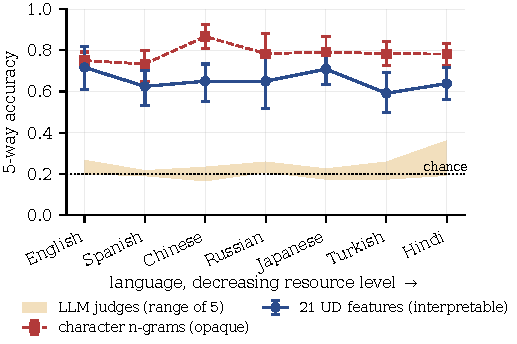
\includegraphics[width=\columnwidth]{fig1_accuracy.pdf}
\caption{Five-way attribution accuracy by language (LOPO, prompt-clustered 95\% CIs). The opaque $n$-gram baseline is more accurate within every language; neither representation declines with resource level; the five LLM judges stay near chance.}
\label{fig:acc}
\end{figure}

\section{Results}
\subsection{RQ1: Attribution works in every language}
Table~\ref{tab:main} and Fig.~\ref{fig:acc} show five-way accuracy of \LRmin{}--\LRmax{} in every language; every prompt-clustered interval excludes chance and every Holm-corrected binomial has $p < 10^{-4}$. Per-model recall is highest for GPT-5.5 (\RecallgptMin{}--\RecallgptMax{} across languages) and Grok 4.3 (\RecallgrokMin{}--\RecallgrokMax{}), then Claude Opus 4.7 (\RecallclaudeMin{}--\RecallclaudeMax{}) and Gemini 3.5 Flash (\RecallgeminiMin{}--\RecallgeminiMax{}); DeepSeek V4 Pro is hardest (\RecalldeepseekMin{}--\RecalldeepseekMax{}). Length is part of the signal: Grok writes the shortest responses in all seven languages. With features residualized on length, logistic regression falls to \LRlenMin{}--\LRlenMax{} while the random forest, which the plan reserves as a ceiling, stays at \RFlenMin{}--\RFlenMax{}; we read this, exploratorily, as a length-independent but non-linear fingerprint.

\textbf{The baseline is more accurate.} Character $n$-grams reach \NGmin{}--\NGmax{} (Table~\ref{tab:main}), \GapNGmin{}--\GapNGmax{} points above the features; word $n$-grams average \WGmean{}. After Holm correction the $n$-gram advantage is significant in \NGsigN{} of seven languages (\NGsigLangs{}) and not in the others. This is the expected result~\cite{sapkota2015ngrams}: $n$-grams see vocabulary, and the interpretable model does not. What the features give up within a language they recover across languages (Sec.~\ref{sec:rq3}) and under translation (Sec.~\ref{sec:rq5}).

\textbf{Feature economy.} By mean absolute coefficient the fingerprint is carried mainly by \TopCoefFeatures{}. The nested selection curve (Fig.~\ref{fig:curve}) shows five features already reach macro-F1 \CurveKfiveMin{}--\CurveKfiveMax{} and ten come within \CurveKtenWithin{} points of all \NFeatures{} in every language; the pooled ranking is \PooledTopFive{}. No feature group is necessary: dropping any one costs at most \AblMaxDrop{} macro-F1, and structure alone gives \AblStructMin{}--\AblStructMax{}, punctuation alone \AblPunctMin{}--\AblPunctMax{}. A character model that sees only punctuation, digits and whitespace, with every word replaced by a placeholder, attributes at \PunctDiag{} within language, direct evidence that the fingerprint is structural.

\begin{figure}[t]
\centering
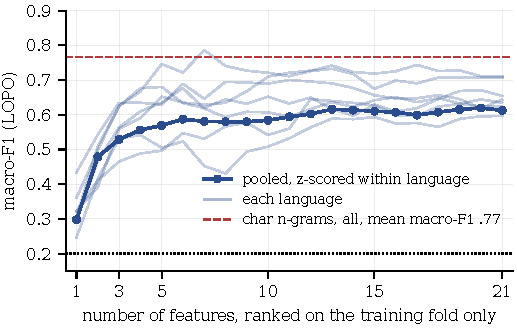
\includegraphics[width=\columnwidth]{fig3_curve.pdf}
\caption{Nested feature-selection curve. Features are ranked on the training fold only; five features carry most of the signal.}
\label{fig:curve}
\end{figure}

\subsection{RQ2: No detectable resource gradient}
The cell-level GLM gives $\beta = \Beta{}$ log-odds per rank step (SE \BetaSE{}, 95\% CI \BetaLo{} to \BetaHi{}, \BetaP{} clustered by prompt; \BetaLangP{} clustered by language; \BetaLangPromptP{} by both). The interval is compatible with a decline of up to \SteepestDeclinePts{} accuracy points from English to Hindi, so the result is a null with bounded power, not a demonstration of invariance. The point estimate is under one accuracy point per step, and the ordering is not monotone: Japanese (rank 5) matches English, and Hindi (rank 7) is more identifiable than Spanish and Turkish. With length-residualized features $\beta = \BetaLen{}$ (\BetaLenP{}); Spearman's $\rho$ over the seven languages is \RhoRQtwo{} (\RhoRQtwoP{}). The $n$-gram baseline shows no gradient either: Hindi (\NGhi{}) exceeds English (\NGen{}), $\rho = \NGrho{}$. Our pre-specified criterion for a gradient (negative coefficient, $p < 0.05$) is not met by either representation.

\subsection{RQ3: A shared fingerprint with a language accent}
\label{sec:rq3}
Averaged over the \NFeatures{} features, partial $\eta^2$ is \EtaLang{} for language, \EtaModel{} for model, \EtaInter{} for the model $\times$ language interaction and \EtaPrompt{} for prompt. Language dominates every feature tied to morphology or vocabulary (token length \EtaLangmeantokenlen{}, function-word ratio \EtaLangfuncwordratio{}, hapax rate \EtaLanghapaxrate{}, Zipf slope \EtaLangzipfslope{}, MATTR \EtaLangmattr{}). Model effects are largest for hapax rate (\EtaModelhapaxrate{}), Zipf slope (\EtaModelzipfslope{}), comma rate (\EtaModelcommaper1k{}), bigram entropy (\EtaModelbigramentropy{}) and paragraph count (\EtaModelparacount{}), and smallest for subordination, question rate and dependency depth ($\leq \EtaModelSmallMax{}$): the models differ in how varied their vocabulary is and how they punctuate and paragraph, not in clause structure.

Removing each language's mean exposes the shared part (Fig.~\ref{fig:transfer}, left). A classifier trained on any language reaches \TransferMin{}--\TransferMax{} on any other (mean \TransferOff{}, against \TransferDiag{} within language), and all \TransferSig{} off-diagonal cells exceed chance after Holm correction. About \TransferRatio{} of within-language accuracy transfers. Given the same unlabelled adaptation, the $n$-gram classifier transfers at mean \NGFairOff{} (Fig.~\ref{fig:transfer}, right), with \NGFairAbove{} of 42 cells above chance; without it, with vocabulary from the training language only, it transfers at \NGTransferOff{}, and \NGTransferConst{} of the 42 cells are constant predictions because no character sequence is shared across scripts. The features are not the only representation that transfers, but they transfer more, and they need no target-language text to do so. The transfer setting is transductive in one respect: the test language's own means and standard deviations (no labels) standardize its features, and all seven language versions share the same 12 prompts.

\begin{figure*}[t]
\centering
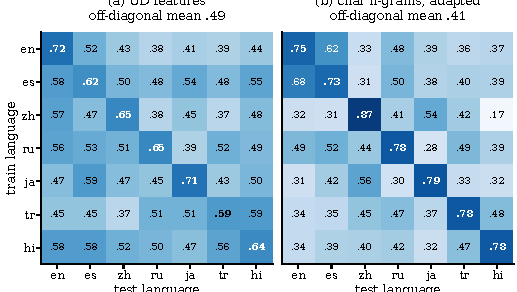
\includegraphics[width=0.96\textwidth]{fig2_transfer.pdf}
\caption{Cross-lingual transfer. A classifier trained on one language (rows) is tested on another (columns) after within-language z-scoring; diagonal: leave-one-prompt-out within language. Left: UD features. Right: character $n$-grams given the same adaptation (union vocabulary, z-scored per language).}
\label{fig:transfer}
\end{figure*}

\subsection{RQ4: Models converge where data is thin}
All three separation measures fall with resource rank. Mean centroid distance drops from \CentEn{} in English to \CentHi{} in Hindi ($\rho = \CentRho{}$, \CentP{}) and the Hindi interval lies below the English one; the between/within scatter ratio falls from \BWen{} to \BWhi{} ($\rho = \BWrho{}$) with intervals also separated; the silhouette falls from \SilEn{} to \SilHi{} ($\rho = \SilRho{}$, \SilP{}), a change within noise of zero, so the pre-registered rule (all three intervals separated) is met for two measures of three. Pairwise distances locate the change: the largest English gaps, GPT--Grok (\PairgptgrokEn{}), Claude--Grok (\PairclaudegrokEn{}) and DeepSeek--Grok (\PairdeepseekgrokEn{}), shrink to \PairgptgrokHi{}, \PairclaudegrokHi{} and \PairdeepseekgrokHi{} in Hindi. Grok's terse, lightly punctuated English register is the outlier that disappears; the other four were never far apart. Convergence and stable attribution are compatible: centroid distance averages over all \NFeatures{} features, most of which converge, while a classifier needs only the few that keep separating the models.

\subsection{RQ5: Translation does not launder the fingerprint}
\label{sec:rq5}
Attribution on translated text alone runs \TrAllMin{}--\TrAllMax{} (Table~\ref{tab:trans}), every interval excluding chance; translating costs about nine points relative to the English originals (\LRen{}), roughly what moving from English to a native lower-resource language costs. A classifier trained on the English originals reads the translations at \TrGoogleTrainEn{} (Google) and \TrLLMTrainEn{} (LLM), while one trained on the models' own native responses in the target language reads them at only \TrGoogleTrainNative{}--\TrLLMTrainNative{}: translated GPT-5.5 text resembles English GPT-5.5 more than native Spanish GPT-5.5, because the translator carries over the source's structural habits. Fig.~\ref{fig:surv} shows why: paragraph count ($\rho = \Survparacount{}$), paragraph length (\Survparalenmean{}), sentence length (\Survsentlenmean{}) and burstiness (\Survburstiness{}) pass through translation almost unchanged, while MATTR (\Survmattr{}), function-word ratio (\Survfuncwordratio{}) and bigram entropy (\Survbigramentropy{}) are rewritten by the target language. The two translators behave almost identically.

$n$-grams retrained on the translations attribute them well (\NGTrLopoMin{}--\NGTrLopoMax{}), but an English-trained $n$-gram model applied across the boundary collapses to \NGTrTrainEnNonLatinMin{}--\NGTrTrainEnNonLatinMax{} on every non-Latin script (\NGTrTrainEnEs{} on Spanish, which shares the alphabet). Only the interpretable features carry a classifier across a translation boundary without retraining. This extends the English-to-Chinese translation result of~\cite{sun2025idiosyncrasies} to six languages, two translators and a representation whose surviving components can be named.

\begin{table}[t]
\caption{Attribution after machine translation of the 120 English responses into six languages (LLM: MiniMax M3). ``Trained on'' rows test on the translations. Reference: English originals \LRen{}; native responses in the six languages, mean \TrNativeMean{}.}
\label{tab:trans}
\centering
\small
\begin{tabular}{l c c}
\toprule
 & Google & LLM \\
\midrule
\multicolumn{3}{l}{\emph{UD features}} \\
\quad LOPO on translations, range & \TrGoogleMin{}--\TrGoogleMax{} & \TrLLMMin{}--\TrLLMMax{} \\
\quad LOPO on translations, mean & \TrGoogleMean{} & \TrLLMMean{} \\
\quad Trained on English originals & \TrGoogleTrainEn{} & \TrLLMTrainEn{} \\
\quad Trained on native responses & \TrGoogleTrainNative{} & \TrLLMTrainNative{} \\
\quad Model $\eta^2$, before $\to$ after & \TrGoogleEtaBefore{} $\to$ \TrGoogleEtaAfter{} & \TrLLMEtaBefore{} $\to$ \TrLLMEtaAfter{} \\
\multicolumn{3}{l}{\emph{Character $n$-grams}} \\
\quad LOPO on translations, mean & \multicolumn{2}{c}{\NGTrLopoMean{}} \\
\quad Trained on English originals & \multicolumn{2}{c}{\NGTrTrainEnMean{}} \\
\bottomrule
\end{tabular}
\end{table}

\begin{figure}[t]
\centering
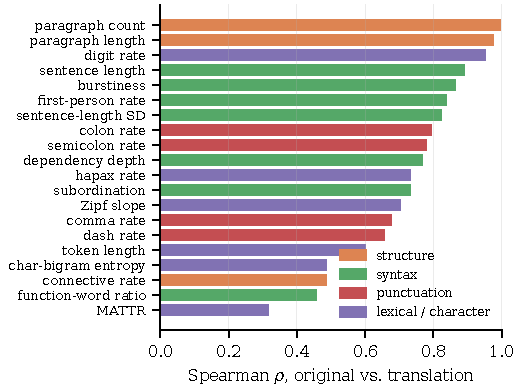
\includegraphics[width=\columnwidth]{fig4_survival.pdf}
\caption{Feature survival under translation. Structural and rhythmic features survive; vocabulary measures are rewritten. Question rate is omitted because the essays contain no questions.}
\label{fig:surv}
\end{figure}

\subsection{RQ6: LLM judges are near chance}
Asked one text at a time which of the five models wrote it, the judges score \Judgedeepseek{} (DeepSeek) to \Judgeclaude{} (Claude). Only Claude is above chance ($p < 10^{-4}$), and only Claude names its own text more often than others' (own-text recall \JudgeclaudeOwn{} vs.\ \JudgeclaudeFalse{} false self-claims; Fisher \JudgeclaudeFisherP{}), the registered prediction. Each judge defaults to one answer: GPT-5.5 names itself for \JudgegptSelfClaim{} of texts regardless of author, Claude most often names GPT-5.5, and the other three most often name Claude. The feature classifier exceeds the best judge by \GapJudgeMin{}--\GapJudgeMax{} points in every language, all Holm-corrected $p < 10^{-4}$. This is the single-text, instant-answer condition; the companion study shows that a side-by-side lineup with reasoning enabled raises the same judges, and Claude's self-recognition in particular, well above these figures~\cite{erlikhman2026compllm}. Claude's best language is Hindi (\ClaudeHindiAcc{}), an exploratory observation across 35 judge--language cells.

\section{Discussion}
Three practical points follow. First, interpretable attribution does not require English: accuracy in Hindi and Turkish is within a few points of Spanish, and a classifier trained in one language transfers to the others. Second, the choice between an opaque and an interpretable representation is a choice about where the classifier will be used. Within one language, with training data in that language, character $n$-grams are the better tool by \GapNGmin{}--\GapNGmax{} points. Across a language or translation boundary, without retraining, they are not usable and the UD features are. Third, machine translation is not an effective way to hide which model wrote a text, because the features that carry the fingerprint are structural, and asking a model who wrote a text is not a substitute for measurement.

The convergence result bears on the homogenization literature~\cite{padmakumar2024diversity,sourati2026shrinking}: model-generated text in lower-resource languages is closer to a shared register than in English. As more of the text in these languages is machine-written, that register may become the default style that readers and future training sets encounter.

\textbf{Dual use.} The same pipeline can attribute text to a person, and the translation result suggests machine translation offers pseudonymous writers little protection against structural stylometry. We release only model-generated text and no tools aimed at human authors.

\textbf{Limitations.} (i) One genre, persuasive essays with a three-claim structure; paragraph count partly reflects instruction following, and other genres may fingerprint differently. (ii) Length is entangled with style; the length-controlled result holds only non-linearly. (iii) Resource level is an ordinal rank over seven languages, and the RQ2 interval admits a decline of up to \SteepestDeclinePts{} points. (iv) Two generations per cell give prompt-clustered intervals of about $\pm$\ClusterCIhalfwidth{} points. (v) Prompt fidelity was checked by a model, not by native speakers. (vi) Parser quality also falls with resource rank and is confounded with it. (vii) Results describe model versions served in September 2026. (viii) Judges were tested without extended reasoning.

\section{Conclusion}
Across seven languages and five frontier models, \NFeatures{} interpretable UD-based features attribute text to its source model at \LRmin{}--\LRmax{} accuracy with no detectable decline in lower-resource languages. A character $n$-gram baseline is more accurate within a language and equally flat across the gradient, but only the interpretable features carry a classifier across languages and through machine translation without retraining, because the fingerprint they capture is structural: five features, led by paragraphing and punctuation, carry most of it. The models' styles converge where training data is thin, and the models themselves cannot read the fingerprint. Future work will test other genres, human-verified prompts, numeric resource covariates and reasoning-enabled judges.

\section*{Data Availability}
Code, native prompts and their reviews, all \NResponses{} analyzed responses, \NTranslations{} translations, \NJudgments{} judge calls, features and every result table: \url{https://github.com/adrian-erlikhman/LangLLM}.

\bibliographystyle{IEEEtran}
\bibliography{references}

\end{document}
